\section{Real-time in embedded Linux systems}

\subsection{Introduction}

\begin{frame}
  \frametitle{Embedded Linux and real time}
  \begin{itemize}
  \item Due to its advantages, Linux and open-source software are more
    and more commonly used in embedded applications
  \item However, some applications also have real-time constraints
  \item They, at the same time, want to
    \begin{itemize}
    \item Get all the nice advantages of Linux: hardware support,
      components re-use, low cost, etc.
    \item Get their real-time constraints met
    \end{itemize}
  \end{itemize}
  \begin{center}
    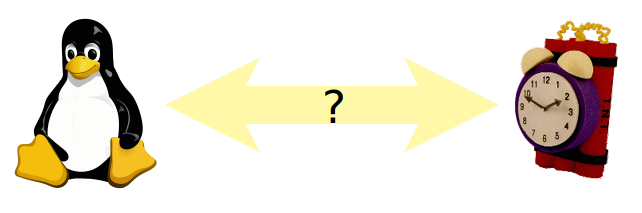
\includegraphics[width=0.5\textwidth]{slides/sysdev-realtime/linux-vs-realtime.pdf}
  \end{center}
\end{frame}

\begin{frame}
  \frametitle{Embedded Linux and real time}
  \begin{itemize}
  \item Linux is an operating system part of the large Unix family
  \item It was originally designed as a time-sharing system
    \begin{itemize}
    \item The main goal was to get the best throughput from the
      available hardware, by making the best possible usage of
      resources (CPU, memory, I/O)
    \item Time determinism was not taken into account
    \end{itemize}
  \item On the opposite, real-time constraints imply time determinism,
    even at the expense of lower global throughput
  \item Best throughput and time determinism are contradictory
    requirements
  \end{itemize}
\end{frame}

\begin{frame}
  \frametitle{Linux and real-time approaches (1)}
  \begin{itemize}
  \item Over time, two major approaches have been taken to bring
    real-time requirements into Linux
  \item {\bf Approach 1}
    \begin{itemize}
    \item Improve the Linux kernel itself so that it matches real-time
      requirements, by providing bounded latencies, real-time APIs,
      etc.
    \item Approach taken by the mainline Linux kernel and the
      {\bf PREEMPT\_RT} project.
    \end{itemize}
  \item {\bf Approach 2}
    \begin{itemize}
    \item Add a layer below the Linux kernel that will handle all the
      real-time requirements, so that the behaviour of Linux doesn't
      affect real-time tasks.
    \item Approach taken by RTLinux, RTAI and {\bf Xenomai}
    \end{itemize}
  \end{itemize}
\end{frame}

\begin{frame}
  \frametitle{Linux and real-time approaches (2)}
  An alternative approach is to use specific hardware to run real-time
  work on:
  \begin{itemize}
  \item Dedicating a CPU core to a real-time OS or to a real-time
        application, using some kind of hypervizor.
  \item Running real-time work on an FPGA
  \item Running real-time work on a dedicated microcontroller.
        For example, the TI AM335x CPU (used in the Beaglebone Black)
        has a "Programmable Real-Time Unit and Industrial
        Communication Subsystem (PRU-ICSS)", which can be used for
        real-time processing.
  \end{itemize}
\end{frame}

\subsection[PREEMPT\_RT Patches]{Improving the main Linux kernel with
  PREEMPT\_RT}

\begin{frame}
  \frametitle{Understanding latency}
  \begin{itemize}
  \item When developing real-time applications with a system such as
    Linux, the typical scenario is the following
    \begin{itemize}
    \item An event from the physical world happens and gets notified
      to the CPU by means of an interrupt
    \item The interrupt handler recognizes and handles the event, and
      then wake-up the user space task that will react to this event
    \item Some time later, the user space task will run and be able to
      react to the physical world event
    \end{itemize}
  \item Real-time is about providing guaranteed worst case latencies
    for this reaction time, called latency
  \end{itemize}
  \begin{center}
    \includegraphics[width=0.9\textwidth]{slides/sysdev-realtime/latency-basic.pdf}
  \end{center}
\end{frame}

\begin{frame}
  \frametitle{Linux kernel latency components}
  \begin{center}
    \includegraphics[width=\textwidth]{slides/sysdev-realtime/latency.pdf}\\
    kernel latency = interrupt latency + handler duration + scheduler
    latency + scheduler duration
  \end{center}
\end{frame}

\begin{frame}
  \frametitle{Interrupt latency}
  \begin{center}
    \includegraphics[width=\textwidth]{slides/sysdev-realtime/latency-highlight-interrupt-latency.pdf}
  \end{center}
\end{frame}

\begin{frame}
  \frametitle{Sources of interrupt latency}
  \begin{itemize}
  \item One of the concurrency prevention mechanism used in the kernel
    is the {\bf spinlock}
  \item It has several variants, but one of the variant commonly used
    to prevent concurrent accesses between a process context and an
    interrupt context works by disabling interrupts
  \item Critical sections protected by spinlocks, or other section in
    which interrupts are explicitly disabled will delay the beginning
    of the execution of the interrupt handler
    \begin{itemize}
    \item The duration of these critical sections is unbounded
    \end{itemize}
  \item Other possible source: shared interrupts (not a real problem:
        mustn't be used for time-critical interrupt-sources anyway).
  \end{itemize}
  \begin{center}
    \includegraphics[width=0.9\textwidth]{slides/sysdev-realtime/spinlock.pdf}
  \end{center}
\end{frame}

\begin{frame}
\frametitle{Interrupt handler duration}
  \begin{center}
    \includegraphics[width=\textwidth]{slides/sysdev-realtime/latency-highlight-interrupt-duration.pdf}
  \end{center}
\end{frame}

\begin{frame}
  \frametitle{Interrupt handler implementation}
  \begin{itemize}
  \item In Linux, many interrupt handlers are split in two parts
    \begin{itemize}
    \item A top-half, started by the CPU as soon as interrupts are
      enabled. It runs with the interrupt line disabled and is
      supposed to complete as quickly as possible.
    \item A bottom-half, scheduled by the top-half, which starts after
      all pending top-halves have completed their execution.
    \end{itemize}
  \item Therefore, for real-time critical interrupts, bottom-halves
    shouldn't be used: their execution is delayed by all other
    interrupts in the system.
  \end{itemize}
  \begin{center}
    \includegraphics[width=0.9\textwidth]{slides/sysdev-realtime/bottom-half-problem.pdf}
  \end{center}
\end{frame}

\begin{frame}
  \frametitle{Scheduler latency}
  \begin{center}
    \includegraphics[width=\textwidth]{slides/sysdev-realtime/latency-highlight-scheduler-latency.pdf}
  \end{center}
\end{frame}

\begin{frame}
  \frametitle{Understanding preemption (1)}
  \begin{itemize}
  \item The Linux kernel is a preemptive operating system
  \item When a task runs in user space mode and gets interrupted by an
    interruption, if the interrupt handler wakes up another task, this
    task can be scheduled as soon as we return from the interrupt
    handler.
  \end{itemize}
  \begin{center}
    \includegraphics[width=0.9\textwidth]{slides/sysdev-realtime/userspace-preemption.pdf}
  \end{center}
\end{frame}

\begin{frame}
  \frametitle{Understanding preemption (2)}
  \begin{itemize}
  \item However, when the interrupt comes while the task is executing
    a system call, this system call has to finish before another task
    can be scheduled.
  \item By default, the Linux kernel does not do kernel preemption.
  \item This means that the time before which the scheduler will be
    called to schedule another task is unbounded.
  \end{itemize}
  \begin{center}
    \includegraphics[width=\textwidth]{slides/sysdev-realtime/kernel-preemption.pdf}
  \end{center}
\end{frame}

\begin{frame}
\frametitle{Scheduler duration}
  \begin{center}
    \includegraphics[width=\textwidth]{slides/sysdev-realtime/latency-highlight-scheduler-duration.pdf}
  \end{center}
\end{frame}

\begin{frame}
  \frametitle{Other non-deterministic mechanisms}
  \begin{itemize}
  \item Outside of the critical path detailed previously, other
    non-deterministic mechanisms of Linux can affect the execution
    time of real-time tasks
  \item Linux is highly based on virtual memory, as provided by an
    MMU, so that memory is allocated on demand. Whenever an
    application accesses code or data for the first time, it is loaded
    on demand, which can creates huge delays.
  \item Many C library services or kernel services are not designed
    with real-time constraints in mind.
  \end{itemize}
\end{frame}

\begin{frame}
  \frametitle{Priority inversion}

  A process with a low priority might hold a lock needed by a higher
  priority process, effectively reducing the priority of this
  process. Things can be even worse if a middle priority process uses
  the CPU.

  \begin{center}
    \includegraphics[width=0.9\textwidth]{slides/sysdev-realtime/priority-inversion.pdf}
  \end{center}
\end{frame}

\begin{frame}
  \frametitle{Interrupt handler priority}

  In Linux, interrupt handlers are executed directly by the CPU
  interrupt mechanisms, and not under control of the Linux
  scheduler. Therefore, all interrupt handlers have a higher priority
  than all tasks running on the system.

  \begin{center}
    \includegraphics[width=0.9\textwidth]{slides/sysdev-realtime/interrupt-inversion.pdf}
  \end{center}
\end{frame}

\begin{frame}
  \frametitle{The PREEMPT\_RT project}
  \begin{itemize}
  \item Long-term project lead by Linux kernel developers Ingo Molnar,
    Thomas Gleixner and Steven Rostedt
    \begin{itemize}
    \item \url{https://rt.wiki.kernel.org}
    \end{itemize}
  \item The goal is to gradually improve the Linux kernel regarding
    real-time requirements and to get these improvements merged into
    the mainline kernel
    \begin{itemize}
    \item PREEMPT\_RT development works very closely with the mainline
      development
    \end{itemize}
  \item Many of the improvements designed, developed and debugged
    inside PREEMPT\_RT over the years are now part of the mainline
    Linux kernel
    \begin{itemize}
    \item The project is a long-term branch of the Linux kernel that
      ultimately should disappear as everything will have been merged
    \end{itemize}
  \end{itemize}
\end{frame}

\begin{frame}
  \frametitle{Improvements in the mainline kernel}
  \begin{columns}[T]
    \column{0.5\textwidth}
    From the PREEMPT\_RT project
    \begin{itemize}
    \item Since the beginning of 2.6
      \begin{itemize}
      \item O(1) scheduler
      \item Kernel preemption
      \item Better POSIX real-time API support
      \end{itemize}
    \item Since 2.6.18
      \begin{itemize}
      \item Priority inheritance support for mutexes
      \end{itemize}
    \end{itemize}
    \column{0.5\textwidth}
    \begin{itemize}
    \item Since 2.6.21
      \begin{itemize}
      \item High-resolution timers
      \end{itemize}
    \end{itemize}
    \begin{itemize}
    \item Since 2.6.30
      \begin{itemize}
      \item Threaded interrupts
      \end{itemize}
    \item Since 2.6.33
      \begin{itemize}
      \item Spinlock annotations
      \end{itemize}
    \end{itemize}
  \end{columns}
  \vspace{0.5cm}
\end{frame}

\begin{frame}
  \frametitle{New preemption options in Linux 2.6}
  2 new preemption models offered by standard Linux 2.6:
  \begin{center}
    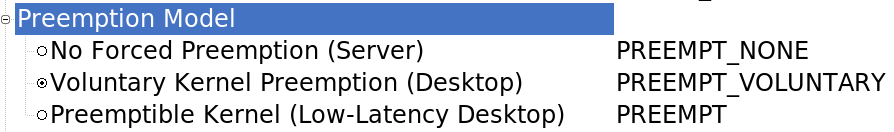
\includegraphics[width=0.9\textwidth]{slides/sysdev-realtime/kernel-config-preemption.png}
  \end{center}
\end{frame}

\begin{frame}
  \frametitle{1st option: no forced preemption}
  \code{CONFIG_PREEMPT_NONE}\\
  Kernel code (interrupts, exceptions, system calls) never preempted.
  Default behavior in standard kernels.
  \begin{itemize}
  \item Best for systems making intense computations, on which overall
    throughput is key.
  \item Best to reduce task switching to maximize CPU and cache usage
    (by reducing context switching).
  \item Still benefits from some Linux 2.6 improvements: O(1)
    scheduler, increased multiprocessor safety (work on RT preemption
    was useful to identify hard to find SMP bugs).
  \item Can also benefit from a lower timer frequency (100 Hz instead
    of 250 or 1000).
  \end{itemize}
\end{frame}

\begin{frame}
  \frametitle{2nd option: voluntary kernel preemption}
  \code{CONFIG_PREEMPT_VOLUNTARY}\\
  Kernel code can preempt itself
  \begin{itemize}
  \item Typically for desktop systems, for quicker application
    reaction to user input.
  \item Adds explicit rescheduling points throughout kernel code.
  \item Minor impact on throughput.
  \item Used in: Ubuntu Desktop 15.04, Ubuntu Server 14.04
  \end{itemize}
\end{frame}

\begin{frame}
  \frametitle{3rd option: preemptible kernel}
  \code{CONFIG_PREEMPT}\\
  Most kernel code can be involuntarily preempted at any time.  When a
  process becomes runnable, no more need to wait for kernel code
  (typically a system call) to return before running the scheduler.
  \begin{itemize}
  \item Exception: kernel critical sections (holding spinlocks).
    In a case you hold a spinlock on a uni-processor system, kernel preemption
    could run another process, which would loop forever if it
    tried to acquire the same spinlock.
  \item Typically for desktop or embedded systems with latency
    requirements in the milliseconds range.
  \item Still a relatively minor impact on throughput.
  \end{itemize}
\end{frame}

\begin{frame}
  \frametitle{Priority inheritance}
  \begin{itemize}
  \item One classical solution to the priority inversion problem is
    called priority inheritance
    \includegraphics[width=0.9\textwidth]{slides/sysdev-realtime/priority-inheritance.pdf}
  \item In Linux, since 2.6.18, mutexes support priority inheritance
  \item In user space, priority inheritance must be explicitly enabled
    on a per-mutex basis.
  \end{itemize}
\end{frame}

\begin{frame}
  \frametitle{High resolution timers}
  \begin{itemize}
  \item The resolution of the timers used to be bound to the
    resolution of the regular system tick
    \begin{itemize}
    \item Usually 100 Hz or 250 Hz, depending on the architecture and
      the configuration
    \item A resolution of only 10 ms or 4 ms.
    \item Increasing the regular system tick frequency is not an
      option as it would consume too many resources
    \end{itemize}
  \item The high-resolution timers infrastructure, merged in 2.6.21,
    allows to use the available hardware timers to program interrupts
    at the right moment.
    \begin{itemize}
    \item Hardware timers are multiplexed, so that a single hardware
      timer is sufficient to handle a large number of
      software-programmed timers.
    \item Usable directly from user space using the usual timer APIs
    \end{itemize}
  \end{itemize}
\end{frame}

\begin{frame}
  \frametitle{Threaded interrupts}
  \begin{itemize}
  \item To solve the interrupt inversion problem, PREEMPT\_RT has
    introduced the concept of threaded interrupts
  \item The interrupt handlers run in normal kernel threads, so that
    the priorities of the different interrupt handlers can be
    configured
  \item The real interrupt handler, as executed by the CPU, is only in
    charge of masking the interrupt and waking-up the corresponding
    thread
  \item The idea of threaded interrupts also allows to use sleeping
    spinlocks (see later)
  \item Merged since 2.6.30, the conversion of interrupt handlers to
    threaded interrupts is not automatic: drivers must be modified
  \item In PREEMPT\_RT, all interrupt handlers are switched to
    threaded interrupts
  \end{itemize}
\end{frame}

\begin{frame}
  \frametitle{The future of the PREEMPT\_RT patchset}
  \begin{itemize}
  \item Before Oct. 2015: project stalled because of the lack of funding.
        Thomas Gleixner still the maintainer but lacked time for further
        development and mainlining efforts. Patch releases only made
        for specific kernel releases.
  \item Oct. 2015: the Linux Foundation at last got funding
        for mainlining the patchset into the Linux kernel (see
        \url{http://lwn.net/Articles/659193/}).
  \item There's at last a good chance for the patchset to be merged
        by the end of 2016.
  \end{itemize}
\end{frame}

\subsection{PREEMPT\_RT specifics}

\begin{frame}
  \frametitle{{\tt CONFIG\_PREEMPT\_RT} (1)}
  \begin{itemize}
  \item The PREEMPT\_RT patch adds a new level of preemption, called
    \code{CONFIG_PREEMPT_RT_FULL}
  \item This level of preemption replaces all kernel spinlocks by
    mutexes (or so-called sleeping spinlocks)
    \begin{itemize}
    \item Instead of providing mutual exclusion by disabling
      interrupts and preemption, they are just normal locks: when
      contention happens, the process is blocked and another one is
      selected by the scheduler.
    \item Works well with threaded interrupts, since threads can
      block, while usual interrupt handlers could not.
    \item Some core, carefully controlled, kernel spinlocks remain as
      normal spinlocks.
    \end{itemize}
  \end{itemize}
\end{frame}

\begin{frame}
  \frametitle{{\tt CONFIG\_PREEMPT\_RT} (2)}
  \begin{itemize}
  \item With \code{CONFIG_PREEMPT_RT_FULL}, virtually all kernel code
    becomes preemptible
    \begin{itemize}
    \item An interrupt can occur at any time, when returning from the
      interrupt handler, the woken up process can start immediately.
    \end{itemize}
  \item This is the last big part of PREEMPT\_RT that isn't fully in
    the mainline kernel yet
    \begin{itemize}
    \item Part of it has been merged in 2.6.33: the spinlock
      annotations. The spinlocks that must remain as spinning
      spinlocks are now differentiated from spinlocks that can be
      converted to sleeping spinlocks. This has reduced a lot the
      PREEMPT\_RT patch size!
    \end{itemize}
  \end{itemize}
\end{frame}

\begin{frame}
  \frametitle{Threaded interrupts}
  \begin{itemize}
  \item The mechanism of threaded interrupts in PREEMPT\_RT is still
    different from the one merged in mainline
  \item In PREEMPT\_RT, all interrupt handlers are unconditionally
    converted to threaded interrupts.
  \item This is a temporary solution, until interesting drivers in
    mainline get gradually converted to the new threaded interrupt API
    that has been merged in 2.6.30.
  \end{itemize}
\end{frame}

\subsection{Setting up PREEMPT\_RT}

\begin{frame}
  \frametitle{PREEMPT\_RT setup (1)}
  \begin{itemize}
  \item PREEMPT\_RT is delivered as a patch against the mainline
    kernel
    \begin{itemize}
    \item Best to have a board supported by the mainline kernel,
      otherwise the PREEMPT\_RT patch may not apply and may require
      some adaptations
    \end{itemize}
  \item Not all releases of the Linux kernel are supported.
      Most recent: 3.10, 3.12, 3.14, 3.18, 4.0, 4.1, 4.4, 4.6, 4.8, 4.9
  \item Quick set up:
    \begin{itemize}
    \item Download the latest PREEMPT\_RT patch\\
      from \footnotesize \url{http://www.kernel.org/pub/linux/kernel/projects/rt/} \normalsize
    \item Download and extract the corresponding mainline kernel
      version
    \item Apply the patch to the mainline kernel tree
    \end{itemize}
  \end{itemize}
\end{frame}

\begin{frame}
  \frametitle{PREEMPT\_RT setup (2)}
  \begin{itemize}
  \item In the kernel configuration, be sure to enable
    \begin{itemize}
    \item \code{CONFIG_PREEMPT_RT_FULL}
    \item High-resolution timers
    \end{itemize}
  \item Compile your kernel, and boot
  \item You are now running the real-time Linux kernel
  \item Of course, some system configuration remains to be done, in
    particular setting appropriate priorities to the interrupt
    threads, which depend on your application.
  \end{itemize}
\end{frame}

\subsection{Real-time application development with PREEMPT\_RT}

\begin{frame}
  \frametitle{Development and compilation}
  \begin{itemize}
  \item No special library is needed, the POSIX real-time API is part
    of the standard C library
  \item The glibc C library is recommended, as support
    for some real-time features is not mature in other C libraries
    \begin{itemize}
    \item Priority inheritance mutexes or NPTL on some architectures,
      for example
    \end{itemize}
  \item Compile a program
    \begin{itemize}
    \item \code{ARCH-linux-gcc -o myprog myprog.c -lrt}
    \end{itemize}
  \item To get the documentation of the POSIX API
    \begin{itemize}
    \item Install the \code{manpages-posix-dev} package
    \item Run \code{man function-name}
    \end{itemize}
  \end{itemize}
\end{frame}

\begin{frame}
  \frametitle{Process, thread?}
  \begin{itemize}
  \item Confusion about the terms {\em process}, {\em thread} and {\em task}
  \item In Unix, a process is created using \code{fork()} and is composed of
    \begin{itemize}
    \item An address space, which contains the program code, data, stack, shared
      libraries, etc.
    \item One thread, that starts executing the \code{main()} function.
    \item Upon creation, a process contains one thread
    \end{itemize}
  \item Additional threads can be created inside an existing process, using
    \code{pthread_create()}
    \begin{itemize}
    \item They run in the same address space as the initial thread of
      the process
    \item They start executing a function passed as argument to
      \code{pthread_create()}
    \end{itemize}
  \end{itemize}
\end{frame}

\begin{frame}
  \frametitle{Process, thread: kernel point of view}
  \begin{itemize}
  \item The kernel represents each thread running in the system by a structure of
    type \code{task_struct}
  \item From a scheduling point of view, it makes no difference
    between the initial thread of a process and all additional threads
    created dynamically using \code{pthread_create()}
  \end{itemize}
  \begin{center}
    \includegraphics[width=0.8\textwidth]{slides/sysdev-realtime/thread-vs-process.pdf}
  \end{center}
\end{frame}

\begin{frame}[fragile]
  \frametitle{Creating threads}
  \begin{itemize}
  \item Linux support the POSIX thread API
  \item To create a new thread
    \begin{block}{}
\small
\begin{verbatim}
pthread_create(pthread_t *thread, pthread_attr_t *attr,
               void *(*routine)(void*), void *arg);
\end{verbatim}
\normalsize
    \end{block}
  \item The new thread will run in the same address space, but will be
    scheduled independently
  \item Exiting from a thread
    \begin{block}{}
\small
\begin{verbatim}
pthread_exit(void *value_ptr);
\end{verbatim}
\normalsize
    \end{block}
  \item Waiting for the termination of a thread
    \begin{block}{}
\small
\begin{verbatim}
pthread_join(pthread_t *thread, void **value_ptr);
\end{verbatim}
\normalsize
    \end{block}
  \end{itemize}
\end{frame}

\begin{frame}
  \frametitle{Scheduling classes (1)}
  \begin{itemize}
  \item The Linux kernel scheduler support different scheduling
    classes
  \item The default class, in which processes are started by default
    is a {\em time-sharing} class
    \begin{itemize}
    \item All processes, regardless of their priority, get some CPU time
    \item The proportion of CPU time they get is dynamic and affected
      by the {\em nice} value, which ranges from -20 (highest) to 19
      (lowest). Can be set using the \code{nice} or \code{renice} commands
    \end{itemize}
  \item The real-time classes \code{SCHED_FIFO} and \code{SCHED_RR}
    \begin{itemize}
    \item The highest priority process gets all the CPU time, until it
      blocks.
    \item In \code{SCHED_RR}, round-robin scheduling between the
      processes of the same priority. All must block before lower
      priority processes get CPU time.
    \item Priorities ranging from 0 (lowest) to 99 (highest)
    \end{itemize}
  \end{itemize}
\end{frame}

\begin{frame}[fragile]
  \frametitle{Scheduling classes (2)}
  \begin{itemize}
  \item An existing program can be started in a specific scheduling
    class with a specific priority using the \code{chrt} command line tool
    \begin{itemize}
    \item Example: \code{chrt -f 99 ./myprog} \\
        \code{-f}: \code{SCHED_FIFO}\\
	\code{-r}: \code{SCHED_RR}
    \end{itemize}
  \item The \code{sched_setscheduler()} API can be used to change the scheduling class
    and priority of a process
    \begin{block}{}
\begin{verbatim}
int sched_setscheduler(pid_t pid, int policy,
                const struct sched_param *param);
\end{verbatim}
    \end{block}{}
    \begin{itemize}
    \item \code{policy} can be \code{SCHED_OTHER}, \code{SCHED_FIFO},
      \code{SCHED_RR}, etc.
    \item \code{param} is a structure containing the priority
    \end{itemize}
  \end{itemize}
\end{frame}

\begin{frame}[fragile]
  \frametitle{Scheduling classes (3)}
  \begin{itemize}
  \item The priority can be set on a per-thread basis when a thread is
    created
    \begin{block}{}
\footnotesize
\begin{verbatim}
struct sched_param parm;
pthread_attr_t attr;

pthread_attr_init(&attr);
pthread_attr_setinheritsched(&attr, PTHREAD_EXPLICIT_SCHED);
pthread_attr_setschedpolicy(&attr, SCHED_FIFO);
parm.sched_priority = 42;
pthread_attr_setschedparam(&attr, &parm);
\end{verbatim}
\normalsize
    \end{block}
  \item Then the thread can be created using \code{pthread_create()},
    passing the \code{attr} structure.
  \item Several other attributes can be defined this way: stack size,
    etc.
  \end{itemize}
\end{frame}

\begin{frame}
  \frametitle{Memory locking}
  \begin{itemize}
  \item In order to solve the non-determinism introduced by virtual
    memory, memory can be locked
    \begin{itemize}
    \item Guarantee that the system will keep it allocated
    \item Guarantee that the system has pre-loaded everything into
      memory
    \end{itemize}
  \item \code{mlockall(MCL_CURRENT | MCL_FUTURE);}
    \begin{itemize}
    \item Locks all the memory of the current address space, for
      currently mapped pages and pages mapped in the future
    \end{itemize}
  \item Other, less useful parts of the API: \code{munlockall}, \code{mlock},
    \code{munlock}.
  \item Watch out for non-currently mapped pages
    \begin{itemize}
    \item Stack pages
    \item Dynamically-allocated memory
    \end{itemize}
  \end{itemize}
\end{frame}

\begin{frame}[fragile]
  \frametitle{Mutexes}
  \begin{itemize}
  \item Allows mutual exclusion between two threads in the same
    address space
  \item Initialization/destruction
    \begin{block}{}
\footnotesize
\begin{verbatim}
pthread_mutex_init(pthread_mutex_t *mutex,
                   const pthread_mutexattr_t *mutexattr);
pthread_mutex_destroy(pthread_mutex_t *mutex);
\end{verbatim}
\normalsize
    \end{block}
  \item Lock/unlock
    \begin{block}{}
\footnotesize
\begin{verbatim}
pthread_mutex_lock(pthread_mutex_t *mutex);
pthread_mutex_unlock(pthread_mutex_t *mutex);
\end{verbatim}
\normalsize
    \end{block}
  \item Priority inheritance must be activated explicitly
    \begin{block}{}
\footnotesize
\begin{verbatim}
pthread_mutexattr_t attr;
pthread_mutexattr_init (&attr);
pthread_mutexattr_setprotocol(&attr, PTHREAD_PRIO_INHERIT);
\end{verbatim}
\normalsize
    \end{block}
  \end{itemize}
\end{frame}

\begin{frame}[fragile]
  \frametitle{Timers}
  \small
  \begin{itemize}
  \item Timer creation
    \begin{block}{}
\footnotesize
\begin{verbatim}
timer_create(clockid_t clockid, struct sigevent *evp,
             timer_t *timerid);
\end{verbatim}
\small
    \end{block}
    \begin{itemize}
    \item \code{clockid} is usually
      \code{CLOCK_MONOTONIC}. \code{sigevent} defines what happens
      upon timer expiration: send a signal or start a function in a
      new thread. \code{timerid} is the returned timer identifier.
    \end{itemize}
  \item Configure the timer for expiration at a given time
    \begin{block}{}
\footnotesize
\begin{verbatim}
timer_settime(timer_t timerid, int flags,
              struct itimerspec *newvalue,
              struct itimerspec *oldvalue);
\end{verbatim}
\small
    \end{block}
  \end{itemize}
\end{frame}

\begin{frame}[fragile]
  \frametitle{Timers (2)}
  \begin{itemize}
  \item Delete a timer
    \begin{block}{}
\footnotesize
\begin{verbatim}
timer_delete(timer_t timerid)
\end{verbatim}
\small
    \end{block}
  \item Get the resolution of a clock, \code{clock_getres}
  \item Other functions: \code{timer_getoverrun()}, \code{timer_gettime()}
  \end{itemize}
\end{frame}


\begin{frame}
  \frametitle{Signals}
  \begin{itemize}
  \item Signals are asynchronous notification mechanisms
  \item Notification occurs either
    \begin{itemize}
    \item By the call of a signal handler. Be careful with the limitations of signal
      handlers!
    \item By being unblocked from the \code{sigwait()},
      \code{sigtimedwait()} or \code{sigwaitinfo()} functions. Usually
      better.
    \end{itemize}
  \item Signal behaviour can be configured using \code{sigaction()}
  \item The mask of blocked signals can be changed with
    \code{pthread_sigmask()}
  \item Delivery of a signal using \code{pthread_kill()} or
    \code{tgkill()}
  \item All signals between \code{SIGRTMIN} and \code{SIGRTMAX}, 32
    signals under Linux.
  \end{itemize}
\end{frame}

\begin{frame}
  \frametitle{Inter-process communication}
  \begin{itemize}
  \item {\bf Semaphores}
    \begin{itemize}
    \item Usable between different processes using named semaphores
    \item \code{sem_open()}, \code{sem_close()}, \code{sem_unlink()},
      \code{sem_init()}, \code{sem_destroy()}, \code{sem_wait()},
      \code{sem_post()}, etc.
    \end{itemize}
  \item {\bf Message queues}
    \begin{itemize}
    \item Allows processes to exchange data in the form of messages.
    \item \code{mq_open()}, \code{mq_close()}, \code{mq_unlink()},
      \code{mq_send()}, \code{mq_receive()}, etc.
    \end{itemize}
  \item {\bf Shared memory}
    \begin{itemize}
    \item Allows processes to communicate by sharing a segment of
      memory
    \item \code{shm_open()}, \code{ftruncate()}, \code{mmap()},
      \code{munmap()}, \code{close()}, \code{shm_unlink()}
    \end{itemize}
  \end{itemize}
\end{frame}

\subsection{Debugging latencies in PREEMPT\_RT}

\begin{frame}
  \frametitle{ftrace - Kernel function tracer}

  Infrastructure that can be used for debugging or analyzing latencies
  and performance issues in the kernel.

  \begin{itemize}
  \item Very well documented in \kerneldoctext{trace/ftrace.txt}
  \item Negligible overhead when tracing is not enabled at run-time.
  \item Can be used to trace any kernel function!
  \end{itemize}
\end{frame}

\begin{frame}
  \frametitle{Using ftrace}
  \begin{itemize}
  \item Tracing information available through the debugfs virtual fs
    (\code{CONFIG_DEBUG_FS} in the {\em Kernel Hacking} section)
  \item Mount this filesystem as follows:\\
    \code{mount -t debugfs nodev /sys/kernel/debug}
  \item When tracing is enabled (see the next slides), tracing
    information is available in \code{/sys/kernel/debug/tracing}.
  \item Check available tracers in
    \code{/sys/kernel/debug/tracing/available_tracers}
  \end{itemize}
\end{frame}

\begin{frame}[fragile]
  \frametitle{Scheduling latency tracer}
  \fontsize{9}{9}\selectfont
  \code{CONFIG_SCHED_TRACER} ({\em Kernel Hacking} section)
  \begin{itemize}
  \item Maximum recorded time between waking up a top priority task
    and its scheduling on a CPU, expressed in us.
  \item Check that \code{wakeup} is listed in
    \code{/sys/kernel/debug/tracing/available_tracers}
  \item To select, reset and enable this tracer:
    \begin{block}{}
\begin{verbatim}
echo wakeup > /sys/kernel/debug/tracing/current_tracer
echo 0 > /sys/kernel/debug/tracing/tracing_max_latency
echo 1 > /sys/kernel/debug/tracing/tracing_enabled
\end{verbatim}
    \end{block}
  \item Let your system run, in particular real-time tasks.\\
    Dummy example: \code{chrt -f 5 sleep 1}
  \item Disable tracing:\\
    \begin{block}{}
\begin{verbatim}
echo 0 > /sys/kernel/debug/tracing/tracing_enabled
\end{verbatim}
    \end{block}{}
  \item Read the maximum recorded latency and the corresponding trace:\\
    \begin{block}{}
\begin{verbatim}
cat /sys/kernel/debug/tracing/tracing_max_latency
\end{verbatim}
    \end{block}{}
  \end{itemize}
\end{frame}
\begin{frame}
  \frametitle{Exemple of worst-case latencies}
  Tests done with \code{cyclictest}
  \begin{itemize}
  \item x86 Geode 500 Mhz: 96 us
  \item x86 Pentium Dual-core T4500 2.3 Ghz: 36 us
  \item ARM Freescale i.MX35 533 Mhz: 120 us
  \item ARM Marvell 88FR131 1200 Mhz: 54 us
  \end{itemize}
  See more results at
  \url{https://www.osadl.org/QA-Farm-Realtime.qa-farm-about.0.html}
\end{frame}

\begin{frame}
  \frametitle{Useful reading}
  About real-time support in the standard Linux kernel
  \begin{itemize}
  \item Inside the RT patch, Steven Rostedt, Red Hat, ELC 2013\\
    \url{http://elinux.org/images/b/ba/Elc2013_Rostedt.pdf}\\
    Video: \url{http://j.mp/1apUtu6}
  \item The Real-Time Linux Wiki: \url{http://rt.wiki.kernel.org}\\
    “The Wiki Web for the CONFIG\_PREEMPT\_RT community, and real-time Linux in general.”\\
    Contains nice and useful documents!
  \item See also our books page.
  \end{itemize}
\end{frame}

\subsection{Real-time extensions to the Linux kernel}

\begin{frame}
  \frametitle{Linux real-time extensions}
  \begin{columns}
    \column{0.5\textwidth}
    Three generations
    \begin{itemize}
    \item RTLinux
    \item RTAI
    \item Xenomai
    \end{itemize}
    \column{0.5\textwidth}
    A common principle
    \begin{itemize}
    \item Add an extra layer between the hardware and the Linux kernel, to manage
      real-time tasks separately.
    \end{itemize}
  \end{columns}
  \begin{center}
    \includegraphics[height=0.4\textheight]{slides/sysdev-realtime/real-time-extensions-architecture.pdf}
  \end{center}
\end{frame}

\begin{frame}
  \frametitle{RTLinux}
  First real-time extension for Linux, created by Victor Yodaiken.
  \begin{itemize}
  \item Nice, but the author filed a software patent covering the
    addition of real-time support to general operating systems as
    implemented in RTLinux!
  \item Its Open Patent License drew many developers away and
    frightened users.  Community projects like RTAI and Xenomai now
    attract most developers and users.
  \item February, 2007: RTLinux rights sold to Wind River. Today,
    no longer advertised by Wind River.
  \item Project completely dead.
  \end{itemize}
\end{frame}

\begin{frame}
  \frametitle{RTAI}
  \url{https://www.rtai.org/} - {\bf Real-Time Application Interface for Linux}
  \begin{itemize}
  \item Created in 1999, by Prof. Paolo Mantegazza (long time
    contributor to RTLinux), Dipartimento di Ingegneria Aerospaziale
    Politecnico di Milano (DIAPM).
  \item Community project. Significant user base. Attracted
    contributors frustrated by the RTLinux legal issues.
  \item Only really actively maintained on x86
  \item May offer slightly better latencies than Xenomai, at the
    expense of a less maintainable and less portable code base
  \item Since RTAI is not really maintained on ARM and other embedded
    architectures, our presentation is focused on Xenomai.
  \end{itemize}
\end{frame}

\begin{frame}
  \frametitle{Xenomai project}
  \begin{columns}[T]
    \column{0.8\textwidth}
    \url{http://www.xenomai.org/}
    \begin{itemize}
    \item Started in 2001 as a project aiming at emulating traditional
      RTOS.
    \item Initial goals: facilitate the porting of programs to GNU /
      Linux.
    \item Initially related to the RTAI project (as the RTAI / fusion
      branch), now independent.
    \item Skins mimicking the APIs of traditional RTOS such as
      VxWorks, pSOS+, and VRTXsa as well as the POSIX API, and a
      “native” API.
    \item Aims at working both as a co-kernel and on top of
      PREEMPT\_RT in future upstream Linux versions.
    \item Will never be merged in the mainline kernel.
    \end{itemize}
    \column{0.2\textwidth}
    
\includegraphics[width=\textwidth]{slides/sysdev-realtime/xenomai.png}
  \end{columns}
\end{frame}

\begin{frame}
  \frametitle{Xenomai architecture}
  \begin{center}
    \includegraphics[width=\textwidth]{slides/sysdev-realtime/xenomai-architecture.pdf}
  \end{center}
\end{frame}

\begin{frame}
  \frametitle{The Adeos interrupt pipeline abstraction}
  \begin{itemize}
  \item From the Adeos point of view, guest OSes are prioritized
    domains.
  \item For each event (interrupts, exceptions, syscalls, etc...), the
    various domains may handle the event or pass it down the pipeline.
  \end{itemize}
  \begin{center}
    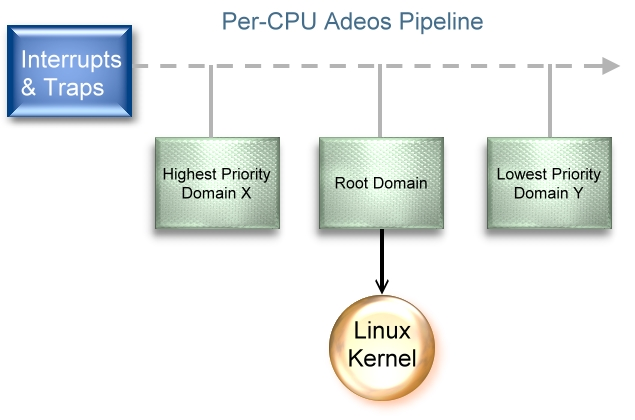
\includegraphics[width=0.7\textwidth]{slides/sysdev-realtime/adeos-interrupt-pipeline1.jpg}
  \end{center}
\end{frame}

\begin{frame}
  \frametitle{Xenomai features}
  \begin{itemize}
  \item Factored real-time core with skins implementing various
    real-time APIs
  \item Seamless support for hard real-time in user space
  \item No second-class citizen, all ports are equivalent feature-wise
  \item Xenomai support is as much as possible independent from the
    Linux kernel version (backward and forward compatible when
    reasonable)
  \item Each Xenomai branch has a stable user/kernel ABI
  \item Timer system based on hardware high-resolution timers
  \item Per-skin time base which may be periodic
  \item RTDM skin allowing to write real-time drivers
  \end{itemize}
\end{frame}

\begin{frame}
  \frametitle{Xenomai user space real-time support}
  \begin{itemize}
  \item Xenomai supports real-time in user space on 5 architectures,
    including 32 and 64 bits variants.
  \item Two modes are defined for a thread
    \begin{itemize}
    \item the primary mode, where the thread is handled by the Xenomai
      scheduler
    \item the secondary mode, when it is handled by the Linux scheduler.
    \end{itemize}
  \item Thanks to the services of the Adeos I-pipe service, Xenomai
    system calls are defined.
    \begin{itemize}
    \item A thread migrates from secondary mode to primary mode when
      such a system call is issued
    \item It migrates from primary mode to secondary mode when a Linux
      system call is issued, or to handle gracefully exceptional
      events such as exceptions or Linux signals.
    \end{itemize}
  \end{itemize}
\end{frame}

\begin{frame}
  \frametitle{Life of a Xenomai application}
  \begin{itemize}
  \item Xenomai applications are started like normal Linux processes,
    they are initially handled by the Linux scheduler and have access
    to all Linux services
  \item After their initialization, they declare themselves as
    real-time applications, which migrates them to primary mode. In
    this mode:
    \begin{itemize}
    \item They are scheduled directly by the Xenomai scheduler, so
      they have the real-time properties offered by Xenomai
    \item They don't have access to any Linux service, otherwise they
      get migrated back to secondary mode and loose all real-time
      properties
    \item They can only use device drivers that are implemented in
      Xenomai, not the ones of the Linux kernel
    \end{itemize}
  \item Need to implement device drivers in Xenomai, and to split
    real-time and non real-time parts of your applications.
  \end{itemize}
\end{frame}

\begin{frame}
  \frametitle{Real Time Driver Model (RTDM)}
  \begin{itemize}
  \item An approach to unify the interfaces for developing device
    drivers and associated applications under real-time Linux
    \begin{itemize}
    \item An API very similar to the native Linux kernel driver API
    \end{itemize}
  \item Allows to develop in kernel space:
    \begin{itemize}
    \item Character-style device drivers
    \item Network-style device drivers
    \end{itemize}
  \item See the whitepaper on\\
    \url{http://www.xenomai.org/documentation/xenomai-2.6/pdf/RTDM-and-Applications.pdf}
  \item Current notable RTDM based drivers:
    \begin{itemize}
    \item Serial port controllers;
    \item RTnet UDP/IP stack;
    \item RT socket CAN, drivers for CAN controllers;
    \item Analogy, fork of the Comedi project, drivers for acquisition cards.
    \end{itemize}
  \end{itemize}
\end{frame}

\subsection{Setting up Xenomai}

\begin{frame}
  \frametitle{How to build Xenomai}
  \begin{itemize}
  \item Download Xenomai sources at
    \url{http://xenomai.org/downloads/xenomai/stable/latest/}
  \item Download one of the Linux versions supported by this release\\
    (see \code{ksrc/arch/<arch>/patches/})
  \item Since version 2.0, split kernel/user building model.
  \item Kernel uses a script called \code{script/prepare-kernel.sh}
    which integrates Xenomai kernel-space support in the Linux
    sources.
  \item Run the kernel configuration menu.
  \end{itemize}
\end{frame}

\begin{frame}
  \frametitle{Linux options for Xenomai configuration}
  \begin{center}
    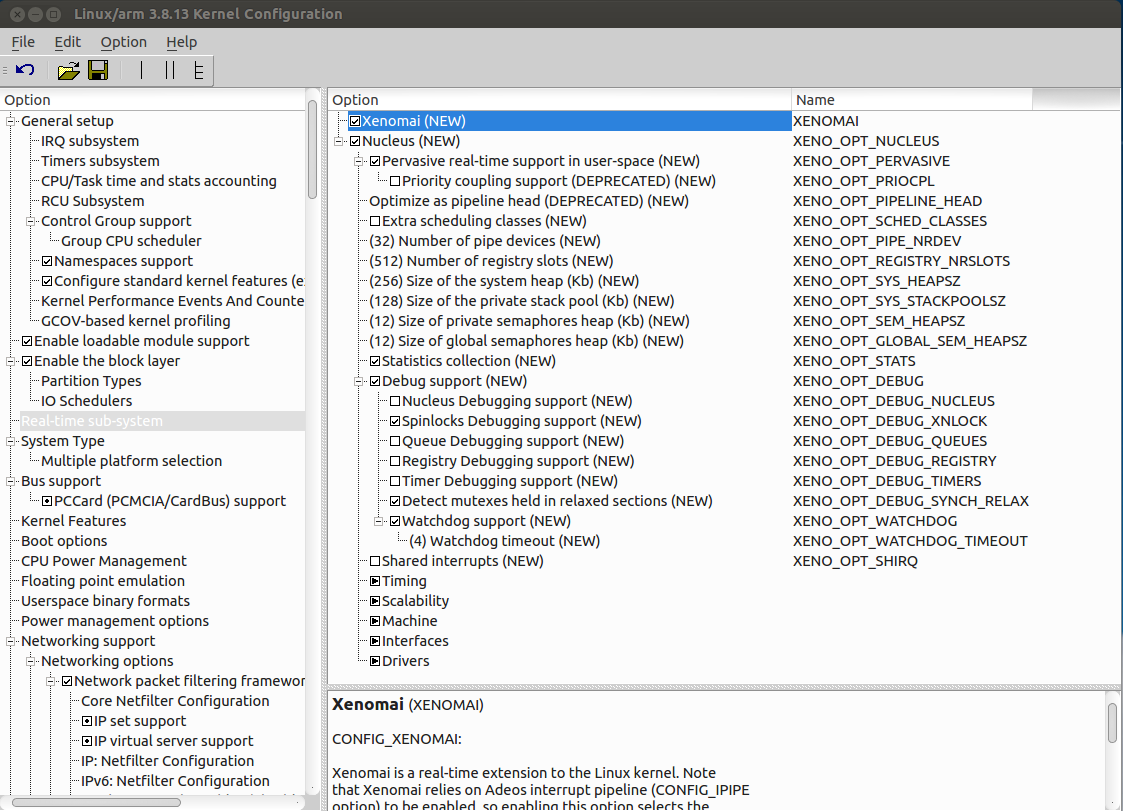
\includegraphics[width=\textwidth]{slides/sysdev-realtime/xenomai-kernel-config.png}
  \end{center}
\end{frame}

\begin{frame}
  \frametitle{Xenomai user space support}
  \begin{itemize}
  \item User space libraries are compiled using the traditional autotools
    \begin{itemize}
    \item \code{./configure --host=arm-linux && make && make DESTDIR=/your/rootfs/ install}
    \end{itemize}
  \item Xenomai installs {\em pkg-config} files which helps you to
    compile your own programs against the Xenomai libraries.
  \item See Xenomai's \code{examples} directory.
  \item Installation details may be found in the \code{README.INSTALL}
    guide.
  \end{itemize}
\end{frame}

\subsection{Developing applications on Xenomai}

\begin{frame}[fragile]
  \frametitle{The POSIX skin}
  \begin{itemize}
  \item The POSIX skin allows to recompile without changes a
    traditional POSIX application so that instead of using Linux
    real-time services, it uses Xenomai services
    \begin{itemize}
    \item {\small
      \url{http://www.xenomai.org/index.php/Porting_POSIX_applications_to_Xenomai}}
    \item Clocks and timers, condition variables, message queues,
      mutexes, semaphores, shared memory, signals, thread management
    \item Good for existing code or programmers familiar with the
      POSIX API
    \end{itemize}
  \item Of course, if the application uses any Linux service that
    isn't available in Xenomai, it will switch back to secondary mode
  \item To link an application against the POSIX skin
  \end{itemize}
  \begin{block}{}
\small
\begin{verbatim}
CFL=`pkg-config --cflags libxenomai_posix`
LDF=`pkg-config --libs libxenomai_posix`
ARCH-gcc $CFL -o rttest rttest.c $LDF
\end{verbatim}
\normalsize
\end{block}
\end{frame}

\begin{frame}[fragile]
  \frametitle{Communication with a normal task}
  \begin{itemize}
  \item If a Xenomai real-time application using the POSIX skin wishes
    to communicate with a separate non-real-time application, it must
    use the rtipc mechanism
  \item In the Xenomai application, create an \code{IPCPROTO_XDDP}
    socket
    \begin{block}{}
\footnotesize
\begin{verbatim}
socket(AF_RTIPC, SOCK_DGRAM, IPCPROTO_XDDP);
setsockopt(s, SOL_RTIPC, XDDP_SETLOCALPOOL,
           &poolsz, sizeof(poolsz));
memset(&saddr, 0, sizeof(saddr));
saddr.sipc_family = AF_RTIPC;
saddr.sipc_port = PORTX;
ret = bind(s, (struct sockaddr *)&saddr, sizeof(saddr));
\end{verbatim}
\normalsize
    \end{block}
    \begin{itemize}
    \item And then the normal socket API \code{sendto()} / \code{recvfrom()}
    \end{itemize}
  \item In the Linux application
    \begin{itemize}
    \item Open \code{/dev/rtpPORTX}, where \code{PORTX} is the XDDP
      port
    \item Use \code{read()} and \code{write()}
    \end{itemize}
  \end{itemize}
\end{frame}

\begin{frame}[fragile]
  \frametitle{The native API (1)}
  \begin{itemize}
  \item A Xenomai specific API for developing real-time tasks
    \begin{itemize}
    \item {\small
      \url{http://xenomai.org/documentation/branches/v2.4.x/pdf/Native-API-Tour-rev-C.pdf}}
    \item Usable both in user space and kernel space. Development of
      tasks in user space is the preferred way.
    \item More coherent and more flexible API than the POSIX
      API. Easier to learn and understand. Certainly the way to go for
      new applications.
    \end{itemize}
  \item Applications should include \code{<native/service.h>}, where
    \code{service} can be \code{alarm}, \code{buffer}, \code{cond},
    \code{event}, \code{heap}, \code{intr}, \code{misc}, \code{mutex},
    \code{pipe}, \code{queue}, \code{sem}, \code{task}, \code{timer}
  \item To compile applications:
    \begin{block}{}
\small
\begin{verbatim}
CFL=`pkg-config --cflags libxenomai_native`
LDF=`pkg-config --libs libxenomai_native`
ARCH-gcc $CFL -o rttest rttest.c $LDF
\end{verbatim}
\normalsize
    \end{block}
  \end{itemize}
\end{frame}

\begin{frame}
  \frametitle{The native API (2)}
  \begin{itemize}
  \item Task management services
    \begin{itemize}
    \item \code{rt_task_create()}, \code{rt_task_start()},
      \code{rt_task_suspend()}, \code{rt_task_resume()},
      \code{rt_task_delete()}, \code{rt_task_join()}, etc.
    \end{itemize}
  \item Counting semaphore services
    \begin{itemize}
    \item \code{rt_sem_create()}, \code{rt_sem_delete()},
      \code{rt_sem_p()}, \code{rt_sem_v()}, etc.
    \end{itemize}
  \item Message queue services
    \begin{itemize}
    \item \code{rt_queue_create()}, \code{rt_queue_delete()},
      \code{rt_queue_alloc()}, \code{rt_queue_free()},
      \code{rt_queue_send()}, \code{rt_queue_receive()}, etc.
    \end{itemize}
  \item Mutex services
    \begin{itemize}
    \item \code{rt_mutex_create()}, \code{rt_mutex_delete()},
      \code{rt_mutex_acquire()}, \code{rt_mutex_release()}, etc.
    \end{itemize}
  \end{itemize}
\end{frame}

\begin{frame}
  \frametitle{The native API (3)}
  \begin{itemize}
  \item Alarm services
    \begin{itemize}
    \item \code{rt_alarm_create()}, \code{rt_alarm_delete()},
      \code{rt_alarm_start()}, \code{rt_alarm_stop()},
      \code{rt_alarm_wait()}, etc.
    \end{itemize}
  \item Memory heap services
    \begin{itemize}
    \item Allows to share memory between processes and/or to
      pre-allocate a pool of memory
    \item \code{rt_heap_create()}, \code{rt_heap_delete()},
      \code{rt_heap_alloc()}, \code{rt_heap_bind()}
    \end{itemize}
  \item Condition variable services
    \begin{itemize}
    \item \code{rt_cond_create()}, \code{rt_cond_delete()},
      \code{rt_cond_signal()}, \code{rt_cond_broadcast()},
      \code{rt_cond_wait()}, etc.
    \end{itemize}
  \end{itemize}
\end{frame}

\begin{frame}
  \frametitle{Xenomai and normal task communication}
  \begin{itemize}
  \item Using {\em rt\_pipes}
  \item In the native Xenomai application, use the Pipe API
    \begin{itemize}
    \item \code{rt_pipe_create()}, \code{rt_pipe_delete()},
      \code{rt_pipe_receive()}, \code{rt_pipe_send()},
      \code{rt_pipe_alloc()}, \code{rt_pipe_free()}
    \end{itemize}
  \item In the normal Linux application
    \begin{itemize}
    \item Open the corresponding \code{/dev/rtpX} file, the minor is specified at
      \code{rt_pipe_create()} time
    \item Then, just \code{read()} and \code{write()} to the opened file
    \end{itemize}
  \end{itemize}
  \begin{center}
    \includegraphics[width=0.9\textwidth]{slides/sysdev-realtime/rtpipe.pdf}
  \end{center}
\end{frame}

\begin{frame}
  \frametitle{Xenomai worst-case latencies results}
  \begin{itemize}
  \item ARM OMAP5432 1.1 GHz: 24 us
  \item ARM OMAP4430 1 GHz: 23 us
  \item ARM OMAP3530 720 MHz: 44 us
  \item ARM SAMA5D3 528 MHz: 51 us
  \item ARM AT91RM9200 180 MHz: 181 us
  \item x86 Atom 1.6 GHz: 35 us
  \item Geode LX800 processor at 500 MHz: 55 us
  \end{itemize}
  See results at \url{http://xenomai.org/~gch/core-3.14-latencies/}
\end{frame}

\begin{frame}
  \frametitle{Books}
  \begin{columns}[T]
    \column{0.8\textwidth}
    {\bf Building Embedded Linux Systems, O'Reilly}\\
    \vspace{0.5cm}
    By Karim Yaghmour, Jon Masters,\\
    Gilad Ben-Yossef, Philippe Gerum and others\\
    (including Michael Opdenacker), August 2008\\
    \vspace{1cm}
    A nice coverage of Xenomai (Philippe Gerum)\\
    and the RT patch (Steven Rostedt)\\
    \vspace{0.5cm}
    \url{http://oreilly.com/catalog/9780596529680/}
    \column{0.2\textwidth}
    
\includegraphics[width=\textwidth]{slides/sysdev-realtime/building-embedded-linux-systems.png}
  \end{columns}
\end{frame}

\begin{frame}
  \frametitle{Organizations}
  \begin{itemize}
  \item \url{http://www.osadl.org}\\
    Open Source Automation Development Lab (OSADL)\\
    Targets machine and plant control systems. Most member companies
    are German (Thomas Gleixner is on board). Supports the use of
    PREEMPT\_RT and Xenomai and contributes to these projects. Shares
    useful documentation and resources.

    They also organize a yearly Real Time Linux Workshop.
  \end{itemize}
\end{frame}

\setuplabframe
{Real-time - Scheduling latency}
{
  \begin{itemize}
  \item Check clock accuracy.
  \item Start processes with real-time priority.
  \item Build a real-time application against the standard POSIX
        real-time API, and against Xenomai’s POSIX skin
  \item Compare scheduling latency on your system, between a standard
        kernel and a kernel with Xenomai.
  \end{itemize}
}

